\documentclass{article}
\usepackage[utf8]{inputenc}
\usepackage{graphicx}
\usepackage{fancyhdr}
\pagestyle{fancy}
\lfoot{\texttt{comsm0094.github.io}}
\lhead{LC\&B - 03.1 Leaky Buckets - Conor}
\rhead{\thepage}
\cfoot{}
\begin{document}

\section*{Leaky buckets}

These notes describe the modelling of a leaky bucket of water,
something that is useful to think about as an analogue of how neurons
behave; both because it is a useful way to think about the equations
and because the actual principles involves are surprisingly similar to
the principles involved in neurons.

\subsection*{Buckets of water}

In the simplest model of neurons their voltage dynamics is similar to
the dynamics of a bucket with a leak and the class of equations that
apply in this case will also be applied to synapses, for example.

%% \begin{center}
%% \setlength{\unitlength}{2mm}
%% \begin{picture}(20,40)
%% \linethickness{0.3mm}
%% \put(7,5){\line(1,0){8}}
%% \put(15,5){\line(0,1){20}}
%% \put(5,5){\line(0,1){20}}
%% \put(15,25){\line(-1,0){10}}
%% \put(6,5){\vector(0,-1){3}}
%% \put(10,27){\vector(0,-1){5}}
%% \put(17,10.5){\vector(0,-1){5.5}}
%% \put(17,14.5){\vector(0,1){5.5}}
%% \linethickness{0.075mm}
%% \put(5,20){\line(1,0){10}}
%% \put(7,2){$l(t)$}
%% \put(11,27){$i(t)$}
%% \put(16,12){$h(t)$}
%% \end{picture}
%% \end{center}

\begin{center}
  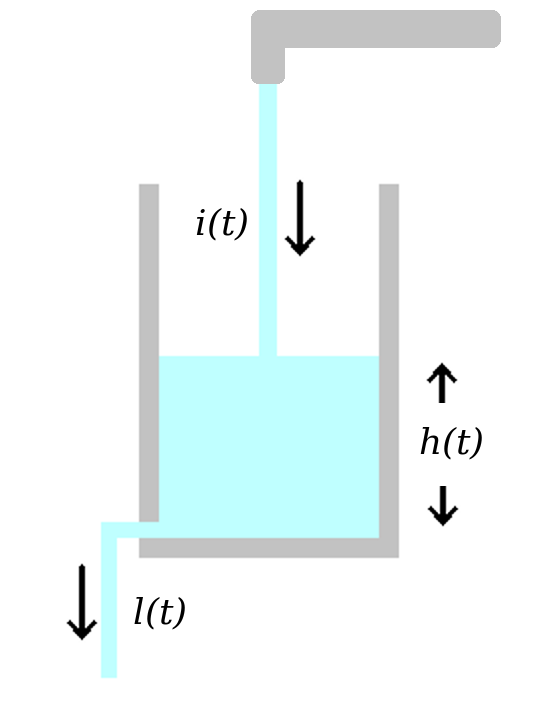
\includegraphics[width=6cm]{glass_notation.png}
  \end{center}


Consider a bucket with straight sides which is filled to a height $h$
with water. Imagine the water leaks out of a hole in the bottom. The
rate the water leaks out depends on $h$; the larger $h$ is the larger
the pressure at the bottom is and hence the faster the water pours
out. In other words
\begin{equation}
l(t)\propto h(t)
\end{equation}
or 
\begin{equation}
l(t)= G h(t)
\end{equation}
where $G$ is a constant which will depend on the size of the hole and
complicated things like the viscosity of water. Of course, we are also
ignoring lots of complicated stuff, like turbulence and so forth, but
since we are interested in the equation rather than the amount of
water in a bucket, this is fine: the main point is that in our model
there is a linear relationship between leak and height. Imagine water
also pours in the top at a rate $i(t)$. This means the total rate of
change of the amount of water is $i(t)-Gh(t)$.

Now, $h(t)$ is the height of the water not the volume: the volume is
$Ch(t)$ where $C$ is the cross-sectional area of the bucket. The rate
of change of the volume is therefore
\begin{equation}
\frac{dCh(t)}{dt}=i(t)-Gh(t)
\end{equation}
or, in other words, the rate the volume of water changes is the difference between the water flowing in and the water flowing out. Divinging across by $G$ this gives
\begin{equation}
\frac{C}{G}\frac{dh}{dt}=\frac{i}{G}-h
\end{equation}
or, if we define $\tau=C/G$ and $y=i/G$
\begin{equation}
\tau\frac{dh}{dt}=y-h
\end{equation}
It is useful to note the dimensions at this point, that is dimensions
in the sense of units: $h$ is a distance, measured in meters or feet
or cubits or whatever, $dh/dt$ in contrast, is distance per time: this
means that $\tau$ has to be timescale for the dimensions to all match. The unit for $\tau$ will be a unit of time, like seconds or whatever.

Let's solve this equation for constant $y$ before going on to look at
neurons: to remind ourselves that we are looking at the constant input
case we'll write $y=\bar{y}$ for the constant values. There are lots
of ways to do this, including Laplace transforms and integrating
factors.  Here we will use an ansatz; ansatz just means guess and what
we do is make a guess as to the solution, the guess will usually have
a few constant in it and we show, by substituing in that we can pick
those constants to make the solution work. Here we use the ansatz:
\begin{equation}
  h(t) = A+ Be^{-rt}
\end{equation}
where $A$, $B$ and $r$ are the constants. There is nothing deep
happening here, I have seen equations like this before so I think I
will be able to find values of the constants that make this a
solution, if I am wrong that won't be possible, though, of course, I
won't be wrong.

So differenciating:
\begin{equation}
  \frac{dh}{dt}=-rBe^{-rt}
\end{equation}
using the rules for differenting exponentials. Substituting that into the equation I get:
\begin{equation}
  -\tau r Be^{-rt} = \bar{y}-A-Be^{-rt}
\end{equation}
For the ansatz to be a solution of the differential equation this
equation needs to hold for all values of $t$ so, basically, it most
hold for the bits multiplying the exponential and for the bits that
don't. Thus
\begin{equation}
  A=\bar{y}
\end{equation}
and
\begin{equation}
  r=1/\tau
\end{equation}
Hence, the ansatz did work and tells us that the equation is solved by
\begin{equation}
  h(t)=\bar{y}+Be^{-t/\tau}
\end{equation}
for any value of $B$. In fact, we can fix this constant using an
initial condition: lets substitute in for $t=0$, the exponential of
zero is one so
\begin{equation}
  h(0)=\bar{y}+B
\end{equation}
and hence
\begin{equation}
  h(t)=\bar{y}+[h(0)-\bar{y}]e^{-t/\tau}
\end{equation}


These dynamics make good intuitive sense; the more water there is in
the bucket, the higher the pressure will be at the leak and the
quicker the water will pour out. If there is just the right amount of
water the rate the water pours out the leak will precisely match the
rate it pours in, this is the equilibrium. If there is more water than
required for equilibrium it will pour out faster than the flow coming
in, if there is less, it will pour out slower. Either way, as time
passes the height of the water will reach the equilibrium. The plot in
Fig.~\ref{bucket_v} illustrates this.

\begin{figure}
\begin{center}
% GNUPLOT: LaTeX picture with Postscript
\begingroup
  \makeatletter
  \providecommand\color[2][]{%
    \GenericError{(gnuplot) \space\space\space\@spaces}{%
      Package color not loaded in conjunction with
      terminal option `colourtext'%
    }{See the gnuplot documentation for explanation.%
    }{Either use 'blacktext' in gnuplot or load the package
      color.sty in LaTeX.}%
    \renewcommand\color[2][]{}%
  }%
  \providecommand\includegraphics[2][]{%
    \GenericError{(gnuplot) \space\space\space\@spaces}{%
      Package graphicx or graphics not loaded%
    }{See the gnuplot documentation for explanation.%
    }{The gnuplot epslatex terminal needs graphicx.sty or graphics.sty.}%
    \renewcommand\includegraphics[2][]{}%
  }%
  \providecommand\rotatebox[2]{#2}%
  \@ifundefined{ifGPcolor}{%
    \newif\ifGPcolor
    \GPcolorfalse
  }{}%
  \@ifundefined{ifGPblacktext}{%
    \newif\ifGPblacktext
    \GPblacktexttrue
  }{}%
  % define a \g@addto@macro without @ in the name:
  \let\gplgaddtomacro\g@addto@macro
  % define empty templates for all commands taking text:
  \gdef\gplbacktext{}%
  \gdef\gplfronttext{}%
  \makeatother
  \ifGPblacktext
    % no textcolor at all
    \def\colorrgb#1{}%
    \def\colorgray#1{}%
  \else
    % gray or color?
    \ifGPcolor
      \def\colorrgb#1{\color[rgb]{#1}}%
      \def\colorgray#1{\color[gray]{#1}}%
      \expandafter\def\csname LTw\endcsname{\color{white}}%
      \expandafter\def\csname LTb\endcsname{\color{black}}%
      \expandafter\def\csname LTa\endcsname{\color{black}}%
      \expandafter\def\csname LT0\endcsname{\color[rgb]{1,0,0}}%
      \expandafter\def\csname LT1\endcsname{\color[rgb]{0,1,0}}%
      \expandafter\def\csname LT2\endcsname{\color[rgb]{0,0,1}}%
      \expandafter\def\csname LT3\endcsname{\color[rgb]{1,0,1}}%
      \expandafter\def\csname LT4\endcsname{\color[rgb]{0,1,1}}%
      \expandafter\def\csname LT5\endcsname{\color[rgb]{1,1,0}}%
      \expandafter\def\csname LT6\endcsname{\color[rgb]{0,0,0}}%
      \expandafter\def\csname LT7\endcsname{\color[rgb]{1,0.3,0}}%
      \expandafter\def\csname LT8\endcsname{\color[rgb]{0.5,0.5,0.5}}%
    \else
      % gray
      \def\colorrgb#1{\color{black}}%
      \def\colorgray#1{\color[gray]{#1}}%
      \expandafter\def\csname LTw\endcsname{\color{white}}%
      \expandafter\def\csname LTb\endcsname{\color{black}}%
      \expandafter\def\csname LTa\endcsname{\color{black}}%
      \expandafter\def\csname LT0\endcsname{\color{black}}%
      \expandafter\def\csname LT1\endcsname{\color{black}}%
      \expandafter\def\csname LT2\endcsname{\color{black}}%
      \expandafter\def\csname LT3\endcsname{\color{black}}%
      \expandafter\def\csname LT4\endcsname{\color{black}}%
      \expandafter\def\csname LT5\endcsname{\color{black}}%
      \expandafter\def\csname LT6\endcsname{\color{black}}%
      \expandafter\def\csname LT7\endcsname{\color{black}}%
      \expandafter\def\csname LT8\endcsname{\color{black}}%
    \fi
  \fi
  \setlength{\unitlength}{0.0500bp}%
  \begin{picture}(5040.00,3528.00)%
    \gplgaddtomacro\gplbacktext{%
      \csname LTb\endcsname%
      \put(946,704){\makebox(0,0)[r]{\strut{} 0}}%
      \put(946,1131){\makebox(0,0)[r]{\strut{} 0.5}}%
      \put(946,1557){\makebox(0,0)[r]{\strut{} 1}}%
      \put(946,1984){\makebox(0,0)[r]{\strut{} 1.5}}%
      \put(946,2410){\makebox(0,0)[r]{\strut{} 2}}%
      \put(946,2837){\makebox(0,0)[r]{\strut{} 2.5}}%
      \put(946,3263){\makebox(0,0)[r]{\strut{} 3}}%
      \put(1078,484){\makebox(0,0){\strut{} 0}}%
      \put(1672,484){\makebox(0,0){\strut{} 0.5}}%
      \put(2266,484){\makebox(0,0){\strut{} 1}}%
      \put(2861,484){\makebox(0,0){\strut{} 1.5}}%
      \put(3455,484){\makebox(0,0){\strut{} 2}}%
      \put(4049,484){\makebox(0,0){\strut{} 2.5}}%
      \put(4643,484){\makebox(0,0){\strut{} 3}}%
      \put(176,1983){\rotatebox{-270}{\makebox(0,0){\strut{}$h(t)$}}}%
      \put(2860,154){\makebox(0,0){\strut{}$t$}}%
    }%
    \gplgaddtomacro\gplfronttext{%
      \csname LTb\endcsname%
      \put(3656,3090){\makebox(0,0)[r]{\strut{}$h(0)=2$}}%
      \csname LTb\endcsname%
      \put(3656,2870){\makebox(0,0)[r]{\strut{}$h(0)=3$}}%
      \csname LTb\endcsname%
      \put(3656,2650){\makebox(0,0)[r]{\strut{}$h(0)=0$}}%
    }%
    \gplbacktext
    \put(0,0){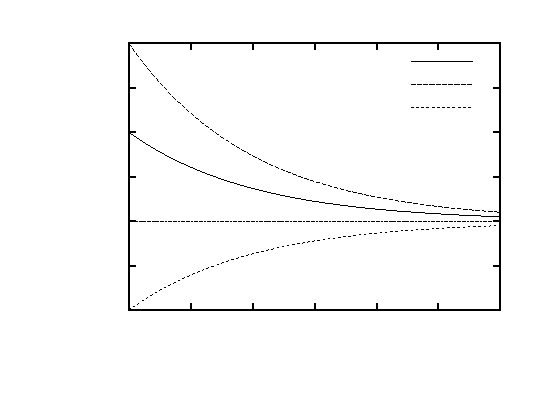
\includegraphics{bucket_v}}%
    \gplfronttext
  \end{picture}%
\endgroup

\end{center}
\caption{Exponential relaxation. The dynamics described by the
  \lq{}bucket equation\rq{} are very common. Here
  $h=[h(0)-\bar{y}]\exp(-t/\tau)+\bar{y}$ is plotted with
  $\tilde{\i}=1$, $\tau=1$ and three different values of
  $h(0)$. $h(t)$ relaxes towards the equilibrium value $\bar{y}=1$,
  the closer it gets, the slower it approaches.\label{bucket_v}}
\end{figure}

\subsection*{Variable input}

We have only discussed constant inputs; the variable input case where
$y$ depends on time is harder and although it can sometimes be solved
it is often easier just to compute it numerically, we will look
briefly at how to do this, but first note that the effect of variable
input is that the solution kind of chases the input with a timescale
set by $\tau$. For very small $\tau$ is chases it quickly, so it is
close to the input, but for large $\tau$ it lags behind it and smooths
it out. This is sometimes described by saying that it \textsl{filters}
the input. There is an illustration in Fig.~\ref{chasing}.

\begin{figure}
\begin{center}
% GNUPLOT: LaTeX picture with Postscript
\begingroup
  \makeatletter
  \providecommand\color[2][]{%
    \GenericError{(gnuplot) \space\space\space\@spaces}{%
      Package color not loaded in conjunction with
      terminal option `colourtext'%
    }{See the gnuplot documentation for explanation.%
    }{Either use 'blacktext' in gnuplot or load the package
      color.sty in LaTeX.}%
    \renewcommand\color[2][]{}%
  }%
  \providecommand\includegraphics[2][]{%
    \GenericError{(gnuplot) \space\space\space\@spaces}{%
      Package graphicx or graphics not loaded%
    }{See the gnuplot documentation for explanation.%
    }{The gnuplot epslatex terminal needs graphicx.sty or graphics.sty.}%
    \renewcommand\includegraphics[2][]{}%
  }%
  \providecommand\rotatebox[2]{#2}%
  \@ifundefined{ifGPcolor}{%
    \newif\ifGPcolor
    \GPcolorfalse
  }{}%
  \@ifundefined{ifGPblacktext}{%
    \newif\ifGPblacktext
    \GPblacktexttrue
  }{}%
  % define a \g@addto@macro without @ in the name:
  \let\gplgaddtomacro\g@addto@macro
  % define empty templates for all commands taking text:
  \gdef\gplbacktext{}%
  \gdef\gplfronttext{}%
  \makeatother
  \ifGPblacktext
    % no textcolor at all
    \def\colorrgb#1{}%
    \def\colorgray#1{}%
  \else
    % gray or color?
    \ifGPcolor
      \def\colorrgb#1{\color[rgb]{#1}}%
      \def\colorgray#1{\color[gray]{#1}}%
      \expandafter\def\csname LTw\endcsname{\color{white}}%
      \expandafter\def\csname LTb\endcsname{\color{black}}%
      \expandafter\def\csname LTa\endcsname{\color{black}}%
      \expandafter\def\csname LT0\endcsname{\color[rgb]{1,0,0}}%
      \expandafter\def\csname LT1\endcsname{\color[rgb]{0,1,0}}%
      \expandafter\def\csname LT2\endcsname{\color[rgb]{0,0,1}}%
      \expandafter\def\csname LT3\endcsname{\color[rgb]{1,0,1}}%
      \expandafter\def\csname LT4\endcsname{\color[rgb]{0,1,1}}%
      \expandafter\def\csname LT5\endcsname{\color[rgb]{1,1,0}}%
      \expandafter\def\csname LT6\endcsname{\color[rgb]{0,0,0}}%
      \expandafter\def\csname LT7\endcsname{\color[rgb]{1,0.3,0}}%
      \expandafter\def\csname LT8\endcsname{\color[rgb]{0.5,0.5,0.5}}%
    \else
      % gray
      \def\colorrgb#1{\color{black}}%
      \def\colorgray#1{\color[gray]{#1}}%
      \expandafter\def\csname LTw\endcsname{\color{white}}%
      \expandafter\def\csname LTb\endcsname{\color{black}}%
      \expandafter\def\csname LTa\endcsname{\color{black}}%
      \expandafter\def\csname LT0\endcsname{\color{black}}%
      \expandafter\def\csname LT1\endcsname{\color{black}}%
      \expandafter\def\csname LT2\endcsname{\color{black}}%
      \expandafter\def\csname LT3\endcsname{\color{black}}%
      \expandafter\def\csname LT4\endcsname{\color{black}}%
      \expandafter\def\csname LT5\endcsname{\color{black}}%
      \expandafter\def\csname LT6\endcsname{\color{black}}%
      \expandafter\def\csname LT7\endcsname{\color{black}}%
      \expandafter\def\csname LT8\endcsname{\color{black}}%
    \fi
  \fi
  \setlength{\unitlength}{0.0500bp}%
  \begin{picture}(7200.00,5040.00)%
    \gplgaddtomacro\gplbacktext{%
      \csname LTb\endcsname%
      \put(726,440){\makebox(0,0)[r]{\strut{}-1}}%
      \put(726,873){\makebox(0,0)[r]{\strut{}-0.8}}%
      \put(726,1307){\makebox(0,0)[r]{\strut{}-0.6}}%
      \put(726,1740){\makebox(0,0)[r]{\strut{}-0.4}}%
      \put(726,2174){\makebox(0,0)[r]{\strut{}-0.2}}%
      \put(726,2608){\makebox(0,0)[r]{\strut{} 0}}%
      \put(726,3041){\makebox(0,0)[r]{\strut{} 0.2}}%
      \put(726,3475){\makebox(0,0)[r]{\strut{} 0.4}}%
      \put(726,3908){\makebox(0,0)[r]{\strut{} 0.6}}%
      \put(726,4342){\makebox(0,0)[r]{\strut{} 0.8}}%
      \put(726,4775){\makebox(0,0)[r]{\strut{} 1}}%
      \put(858,220){\makebox(0,0){\strut{} 0}}%
      \put(1453,220){\makebox(0,0){\strut{} 2}}%
      \put(2047,220){\makebox(0,0){\strut{} 4}}%
      \put(2642,220){\makebox(0,0){\strut{} 6}}%
      \put(3236,220){\makebox(0,0){\strut{} 8}}%
      \put(3831,220){\makebox(0,0){\strut{} 10}}%
      \put(4425,220){\makebox(0,0){\strut{} 12}}%
      \put(5020,220){\makebox(0,0){\strut{} 14}}%
      \put(5614,220){\makebox(0,0){\strut{} 16}}%
      \put(6209,220){\makebox(0,0){\strut{} 18}}%
      \put(6803,220){\makebox(0,0){\strut{} 20}}%
    }%
    \gplgaddtomacro\gplfronttext{%
      \csname LTb\endcsname%
      \put(5816,4602){\makebox(0,0)[r]{\strut{}$\tau=0.25$}}%
      \csname LTb\endcsname%
      \put(5816,4382){\makebox(0,0)[r]{\strut{}$\tau=2$}}%
      \csname LTb\endcsname%
      \put(5816,4162){\makebox(0,0)[r]{\strut{}$\tau=4$}}%
      \csname LTb\endcsname%
      \put(5816,3942){\makebox(0,0)[r]{\strut{}input}}%
    }%
    \gplbacktext
    \put(0,0){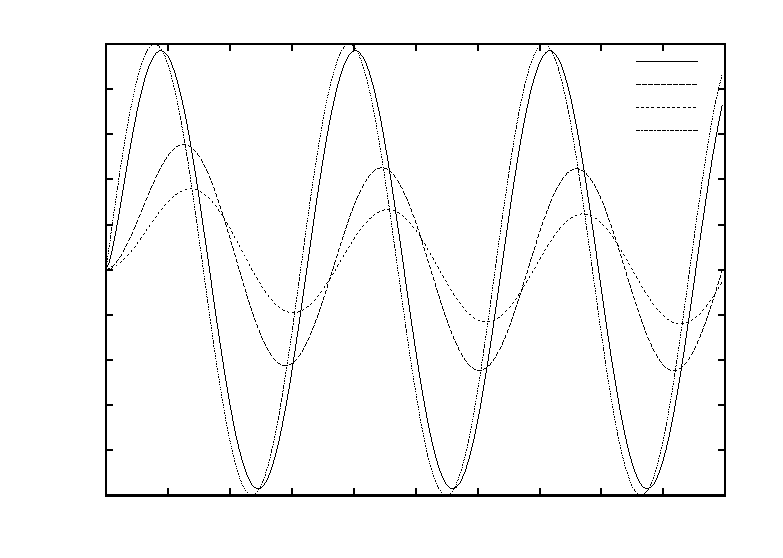
\includegraphics{chasing}}%
    \gplfronttext
  \end{picture}%
\endgroup

\end{center}
\caption{Variable input. Here the input is a sine wave
  $\bar{y}=\sin{t}$ and the equation is evolved with $h(0)$ and three
  different $\tau$ values. For $\tau=0.25$ we see $h(t)$ closely
  matches the input whereas for larger $\tau$ it is smoother and lags
  behind.\label{chasing}}
\end{figure}


\begin{figure}
\begin{center}
% GNUPLOT: LaTeX picture with Postscript
\begingroup
  \makeatletter
  \providecommand\color[2][]{%
    \GenericError{(gnuplot) \space\space\space\@spaces}{%
      Package color not loaded in conjunction with
      terminal option `colourtext'%
    }{See the gnuplot documentation for explanation.%
    }{Either use 'blacktext' in gnuplot or load the package
      color.sty in LaTeX.}%
    \renewcommand\color[2][]{}%
  }%
  \providecommand\includegraphics[2][]{%
    \GenericError{(gnuplot) \space\space\space\@spaces}{%
      Package graphicx or graphics not loaded%
    }{See the gnuplot documentation for explanation.%
    }{The gnuplot epslatex terminal needs graphicx.sty or graphics.sty.}%
    \renewcommand\includegraphics[2][]{}%
  }%
  \providecommand\rotatebox[2]{#2}%
  \@ifundefined{ifGPcolor}{%
    \newif\ifGPcolor
    \GPcolorfalse
  }{}%
  \@ifundefined{ifGPblacktext}{%
    \newif\ifGPblacktext
    \GPblacktexttrue
  }{}%
  % define a \g@addto@macro without @ in the name:
  \let\gplgaddtomacro\g@addto@macro
  % define empty templates for all commands taking text:
  \gdef\gplbacktext{}%
  \gdef\gplfronttext{}%
  \makeatother
  \ifGPblacktext
    % no textcolor at all
    \def\colorrgb#1{}%
    \def\colorgray#1{}%
  \else
    % gray or color?
    \ifGPcolor
      \def\colorrgb#1{\color[rgb]{#1}}%
      \def\colorgray#1{\color[gray]{#1}}%
      \expandafter\def\csname LTw\endcsname{\color{white}}%
      \expandafter\def\csname LTb\endcsname{\color{black}}%
      \expandafter\def\csname LTa\endcsname{\color{black}}%
      \expandafter\def\csname LT0\endcsname{\color[rgb]{1,0,0}}%
      \expandafter\def\csname LT1\endcsname{\color[rgb]{0,1,0}}%
      \expandafter\def\csname LT2\endcsname{\color[rgb]{0,0,1}}%
      \expandafter\def\csname LT3\endcsname{\color[rgb]{1,0,1}}%
      \expandafter\def\csname LT4\endcsname{\color[rgb]{0,1,1}}%
      \expandafter\def\csname LT5\endcsname{\color[rgb]{1,1,0}}%
      \expandafter\def\csname LT6\endcsname{\color[rgb]{0,0,0}}%
      \expandafter\def\csname LT7\endcsname{\color[rgb]{1,0.3,0}}%
      \expandafter\def\csname LT8\endcsname{\color[rgb]{0.5,0.5,0.5}}%
    \else
      % gray
      \def\colorrgb#1{\color{black}}%
      \def\colorgray#1{\color[gray]{#1}}%
      \expandafter\def\csname LTw\endcsname{\color{white}}%
      \expandafter\def\csname LTb\endcsname{\color{black}}%
      \expandafter\def\csname LTa\endcsname{\color{black}}%
      \expandafter\def\csname LT0\endcsname{\color{black}}%
      \expandafter\def\csname LT1\endcsname{\color{black}}%
      \expandafter\def\csname LT2\endcsname{\color{black}}%
      \expandafter\def\csname LT3\endcsname{\color{black}}%
      \expandafter\def\csname LT4\endcsname{\color{black}}%
      \expandafter\def\csname LT5\endcsname{\color{black}}%
      \expandafter\def\csname LT6\endcsname{\color{black}}%
      \expandafter\def\csname LT7\endcsname{\color{black}}%
      \expandafter\def\csname LT8\endcsname{\color{black}}%
    \fi
  \fi
    \setlength{\unitlength}{0.0500bp}%
    \ifx\gptboxheight\undefined%
      \newlength{\gptboxheight}%
      \newlength{\gptboxwidth}%
      \newsavebox{\gptboxtext}%
    \fi%
    \setlength{\fboxrule}{0.5pt}%
    \setlength{\fboxsep}{1pt}%
\begin{picture}(7200.00,5040.00)%
    \gplgaddtomacro\gplbacktext{%
      \csname LTb\endcsname%%
      \put(594,440){\makebox(0,0)[r]{\strut{}$0$}}%
      \put(594,1024){\makebox(0,0)[r]{\strut{}$0.2$}}%
      \put(594,1608){\makebox(0,0)[r]{\strut{}$0.4$}}%
      \put(594,2192){\makebox(0,0)[r]{\strut{}$0.6$}}%
      \put(594,2775){\makebox(0,0)[r]{\strut{}$0.8$}}%
      \put(594,3359){\makebox(0,0)[r]{\strut{}$1$}}%
      \put(594,3943){\makebox(0,0)[r]{\strut{}$1.2$}}%
      \put(594,4527){\makebox(0,0)[r]{\strut{}$1.4$}}%
      \put(726,220){\makebox(0,0){\strut{}$0$}}%
      \put(1334,220){\makebox(0,0){\strut{}$2$}}%
      \put(1941,220){\makebox(0,0){\strut{}$4$}}%
      \put(2549,220){\makebox(0,0){\strut{}$6$}}%
      \put(3157,220){\makebox(0,0){\strut{}$8$}}%
      \put(3765,220){\makebox(0,0){\strut{}$10$}}%
      \put(4372,220){\makebox(0,0){\strut{}$12$}}%
      \put(4980,220){\makebox(0,0){\strut{}$14$}}%
      \put(5588,220){\makebox(0,0){\strut{}$16$}}%
      \put(6195,220){\makebox(0,0){\strut{}$18$}}%
      \put(6803,220){\makebox(0,0){\strut{}$20$}}%
    }%
    \gplgaddtomacro\gplfronttext{%
      \csname LTb\endcsname%%
      \put(5816,4646){\makebox(0,0)[r]{\strut{}fast}}%
      \csname LTb\endcsname%%
      \put(5816,4426){\makebox(0,0)[r]{\strut{}slow}}%
    }%
    \gplbacktext
    \put(0,0){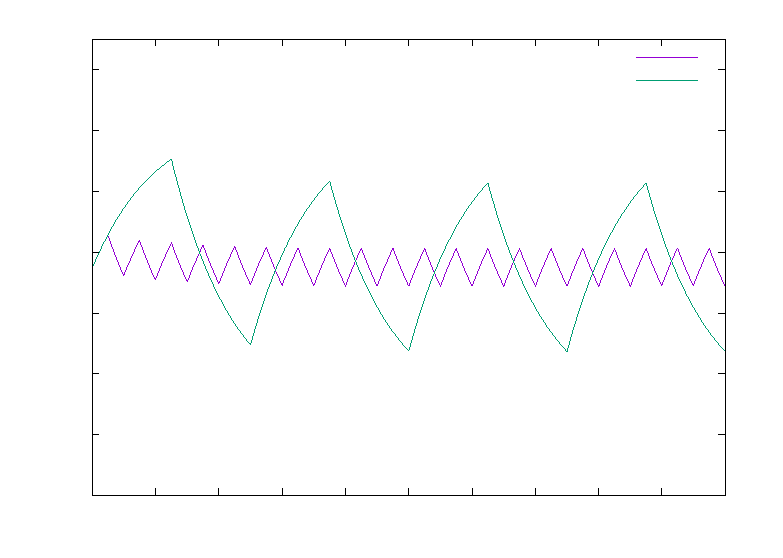
\includegraphics{pw}}%
    \gplfronttext
  \end{picture}%
\endgroup

\end{center}
\caption{Piecewise constant input. Here the input is a function that
  is either $y=0.5$ or $y=1.5$; for \textbf{fast} this flips every 0.5
  so the period is one, for \textbf{slow} it flips ever 2.5 so the
  persion is 5; in both cases $\tau=2$ and the initial $v$ is 0.75.\label{pw}}
\end{figure}


\end{document}

